\chapter{Implementacja}

Założeniem projektu było stworzenie konfigurowalnej platformy umożliwiającej przeprowadzanie testów wydajnościowych dla różnych metod komunikacji międzyprocesowej. Głowna część (silnik testujący) zrealizowana została w oparciu o Javę 9 i jej wirtualną maszynę.

Dane wejściowe to m. in. wybrany sposób komunikacji oraz jego konfiguracja, a także rozmiar danych do wysłania i odbioru. Aplikacja wykona pomiary oraz zapisze wyniki w formacie CSV.

Wartość, która jest istotna to czas jaki zajęła dwukierunkowa komunikacja. Cechuje się ona nanosekundową precyzją, lecz jej rozdzielczość jest większa. Wynika to działania metody \textit{System.nanoTime()} w Javie.

\begin{lstlisting}[caption={Metoda klasy abstrakcyjnej AbstractTransferTester, która jest wykorzysywana przez wszystkie sposoby komunikacji do wykonania pomiarów (implementowane/przeciążane są ostatnie 3 metody).},captionpos=b]
    public Metrics test(TestProps testProps) {
        beforeTest(testProps);
        long start = System.nanoTime();
        try {
            execute(testProps);
        } catch (TesterException e) {
            log.error("TesterException", e);
            afterTest();
            return Metrics.error(testProps.getRequestBytes().length,
                    testProps.getResponseSize(), testType);
        }

        long time = System.nanoTime() - start;
        afterTest();
        return Metrics.of(time, testProps.getRequestBytes().length,
                testProps.getResponseSize(), testType);
    }

    protected void beforeTest(TestProps testProps) {}

    protected abstract void execute(TestProps testProps) throws TesterException;

    protected void afterTest() {}
\end{lstlisting}


Aby zachować wiarygodność testów, przeprowadzone zostały wielokrotnie - każda wykorzystana konfiguracja testowa była wykonana co najmniej 1000-krotnie.

Przed właściwym testowaniem zawsze następowały uruchomienia niepomiarowe, aby \enquote{rozgrzać maszynę writualną}. To znaczy, aby uzyskać pełną wydajność. Celem jest wcześniejsze załadowanie klas do pamięci oraz poczekanie aż JIT (ang. \textit{just-in-time compilation} - kompilacja tuż przed wykonaniem kodu) dokona kompilacji do kodu natywnego oraz optymalizacji.

Charater testów był czysto naukowy. Dane przesyłane w zapytaniach to losowe bajty oraz rozmiar oczekiwanej odpowiedzi, aby dynamicznie sterować wielkościami komunikatów - bez rekonfigurowania serwerów oczekujących na klienta.

Odpowiedź generowana po stronie implementowanej w C/C++ została ujednolicona, tak aby nie fałszować różnic między metodami transportu.

\begin{lstlisting}[caption={Fragment kodu wykorzystywanego w każdej metodzie komunikacji do generowania odpowiedzi},captionpos=b]
    for (int i = 0; i < responseSize; i++) {
        response[i] = (i % 26) + 65;
    }
\end{lstlisting}

W kolejnych sekcjach przybliżony zostanie sposób testowania poszczególnych metod komunikacji. Platformą docelową dla wszystkich implementacji jest Linux - na nim przeprowadzone zostały wszystkie uruchomienia (mimo że większość wspiera także macOS oraz Windows).

\section{TCP}

Zaimplementowany został własny protokół służący badaniu szybkości transferu danych oparty o gniazda TCP. Aby klient mógł zlokalizować serwer potrzebny jest mu jego adres IP i port oraz oczywiście musi istnieć możliwość stworzenia trasy.

Strona serwerowa wykorzystuje bibliotekę \texttt{unistd.h}. Klient opiera się o~standardową bibliotekę Javy, czyli klasę \texttt{java.net.Socket}.

\begin{figure}[h!]
	\centering
	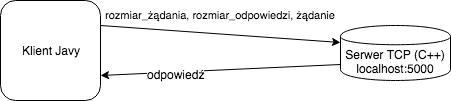
\includegraphics{img/tcp_diagram.png}
	\caption{Diagram prezentujący działanie własnego protokołu opartego na TCP}
\end{figure}

Sam protokół jest typu żądanie/odpowiedź - to znaczy za każdym razem otwierane jest gniazdo, a po otrzymaniu odpowiedzi zamykane. Jego działanie wygląda następująco:
\newline
Klient wysyła wiadomość składającą się kolejno z:
\begin{enumerate}
    \item 4 bajtów rozmiaru żądania
    \item 4 bajtów rozmiaru oczekiwanej odpowiedzi
    \item bajtów żądania w rozmiarze określonym na początku
\end{enumerate}
Serwer odpowiada bajtami odpowiedzi w rozmiarze określonym przez klienta (sam je generuje).


\section{REST}

REST TODO


\section{pliki}

Pliki TODO


\section{CORBA}

CORBA TODO


\section{JNI}

JNI TODO


\section{tmp}

- testy na sucho (mock) w celu sprawdzenia narzutu samej platformy
- obrazek architektury klientów (może per metoda komunikacji?)
- grupowanie danych po nanosekundach, req size, res size, test type
- wykorzystane biblioteki?
- rozmiar każdej z technologi (np. linie kodu, rozmiar)

+ testy powatarzane wielokrotnie, aby uniknąć skrajnych wyników
+ na początku niemierzone testy, aby rozgrzać JVM
+ snippet generowania responsa używany w C/C++
+ sekcja per metoda komunikacji (TCP, REST, komunikacja przez pliki, CORBA, JNI)

wnioski z testow:
- dokladny opis platformy (system, sprzęt)
- wykresy